\chapter{Background}

\section{GPUs}

%Without loss of generality, this thesis will use the NVIDIA and OpenCL definitions and \acrshort{gpu} terminology.

\Acrfullpl{gpu} are accelerators designed for executing highly parallelizable workloads. They are able to achieve high throughput by exploiting \acrfull{simt}. GPUs have a number of \acrfullpl{sm}, each with a set of parallel execution lanes, which can execute a set of logically independent threads. These threads are all a part of the same program known as the kernel. The programming model of GPUs is \textit{data-parallel}, that is the program is divided into a set of threads, all executing the same program, but with different data. As illustrated in Figure \ref{fig:kernel_work_items}, the kernel is divided into threads which is grouped into blocks called \acrfullpl{tb}. These \acrshortpl{tb} are then allocated and executed on the \acrshortpl{sm} in the \acrshort{gpu}. The \acrshortpl{sm} can be allocated a number of \acrshortpl{tb} at the same time. During execution, each \acrshort{sm} can execute \textit{warps} from all of its allocated \acrshortpl{tb}. A \textit{warp} is the next instruction in a \acrshort{tb} and is the basic execution unit of the \acrshort{gpu}. The threads within a warp run in lock-step, this means that all the threads execute the same instruction. In the case of divergence between threads, the branching threads are disabled, while the non-branching threads continue execution until their paths rejoin.

By having multiple \acrshortpl{tb} allocated to each \acrshort{sm}, the \acrshortpl{gpu} can hide stalls by interleaving their warps. As \acrshortpl{sm} have multiple \acrfullpl{fu} to execute instructions, it is likely that if a warp stalls a warp from another \acrshort{tb} is able to execute. This results in a high degree of \acrfull{tlp} and \acrfull{mlp}. Due to the amount of \acrshort{mlp}, \acrshortpl{gpu} require high memory bandwidth\cite{get_out_of_the_valley}. \acrshort{mlp} allows \acrshortpl{gpu} to hide memory latency and obtain high throughput.

When a kernel is executed on a \acrshort{gpu}, the \acrshortpl{tb} have to be divided among the \acrshortpl{sm}. This is the job of the \acrshort{tb} scheduler. The \acrshort{tb} scheduler attempts to balance the workload evenly among the \acrshortpl{sm} during execution. Figure \ref{fig:tb_scheduler} shows an example of how a \acrshort{tb} scheduler might distribute \acrshortpl{tb} among \acrshortpl{sm}. For Nvidia \acrshortpl{gpu}, it attempts to maximize \acrshort{tb} occupancy\cite{CTA_scheduling}, i.e maximize the number of \acrshortpl{tb} in \acrshortpl{sm} at all times. This is done by periodically obtaining information from every \acrshort{sm} regarding the available resources over a dedicated network, and selecting the \acrshort{sm} best fit for the next \acrshort{tb}. The \acrshort{tb} scheduler can account for factors such as data locality when selecting the best fitting \acrshort{sm}. In the case of clustered \acrshortpl{sm}, the \acrshort{tb} scheduler can also aim at distributing \acrshortpl{tb} evenly among the clusters, or map close \acrshortpl{tb} to the same cluster \cite{wang2020modeling}. Having good load balancing will allow the \acrshortpl{sm} to execute the kernel efficiently and balance the load evenly to obtain high utilization of the \acrshortpl{sm} and reduce idling.

\begin{figure}
    \centering
    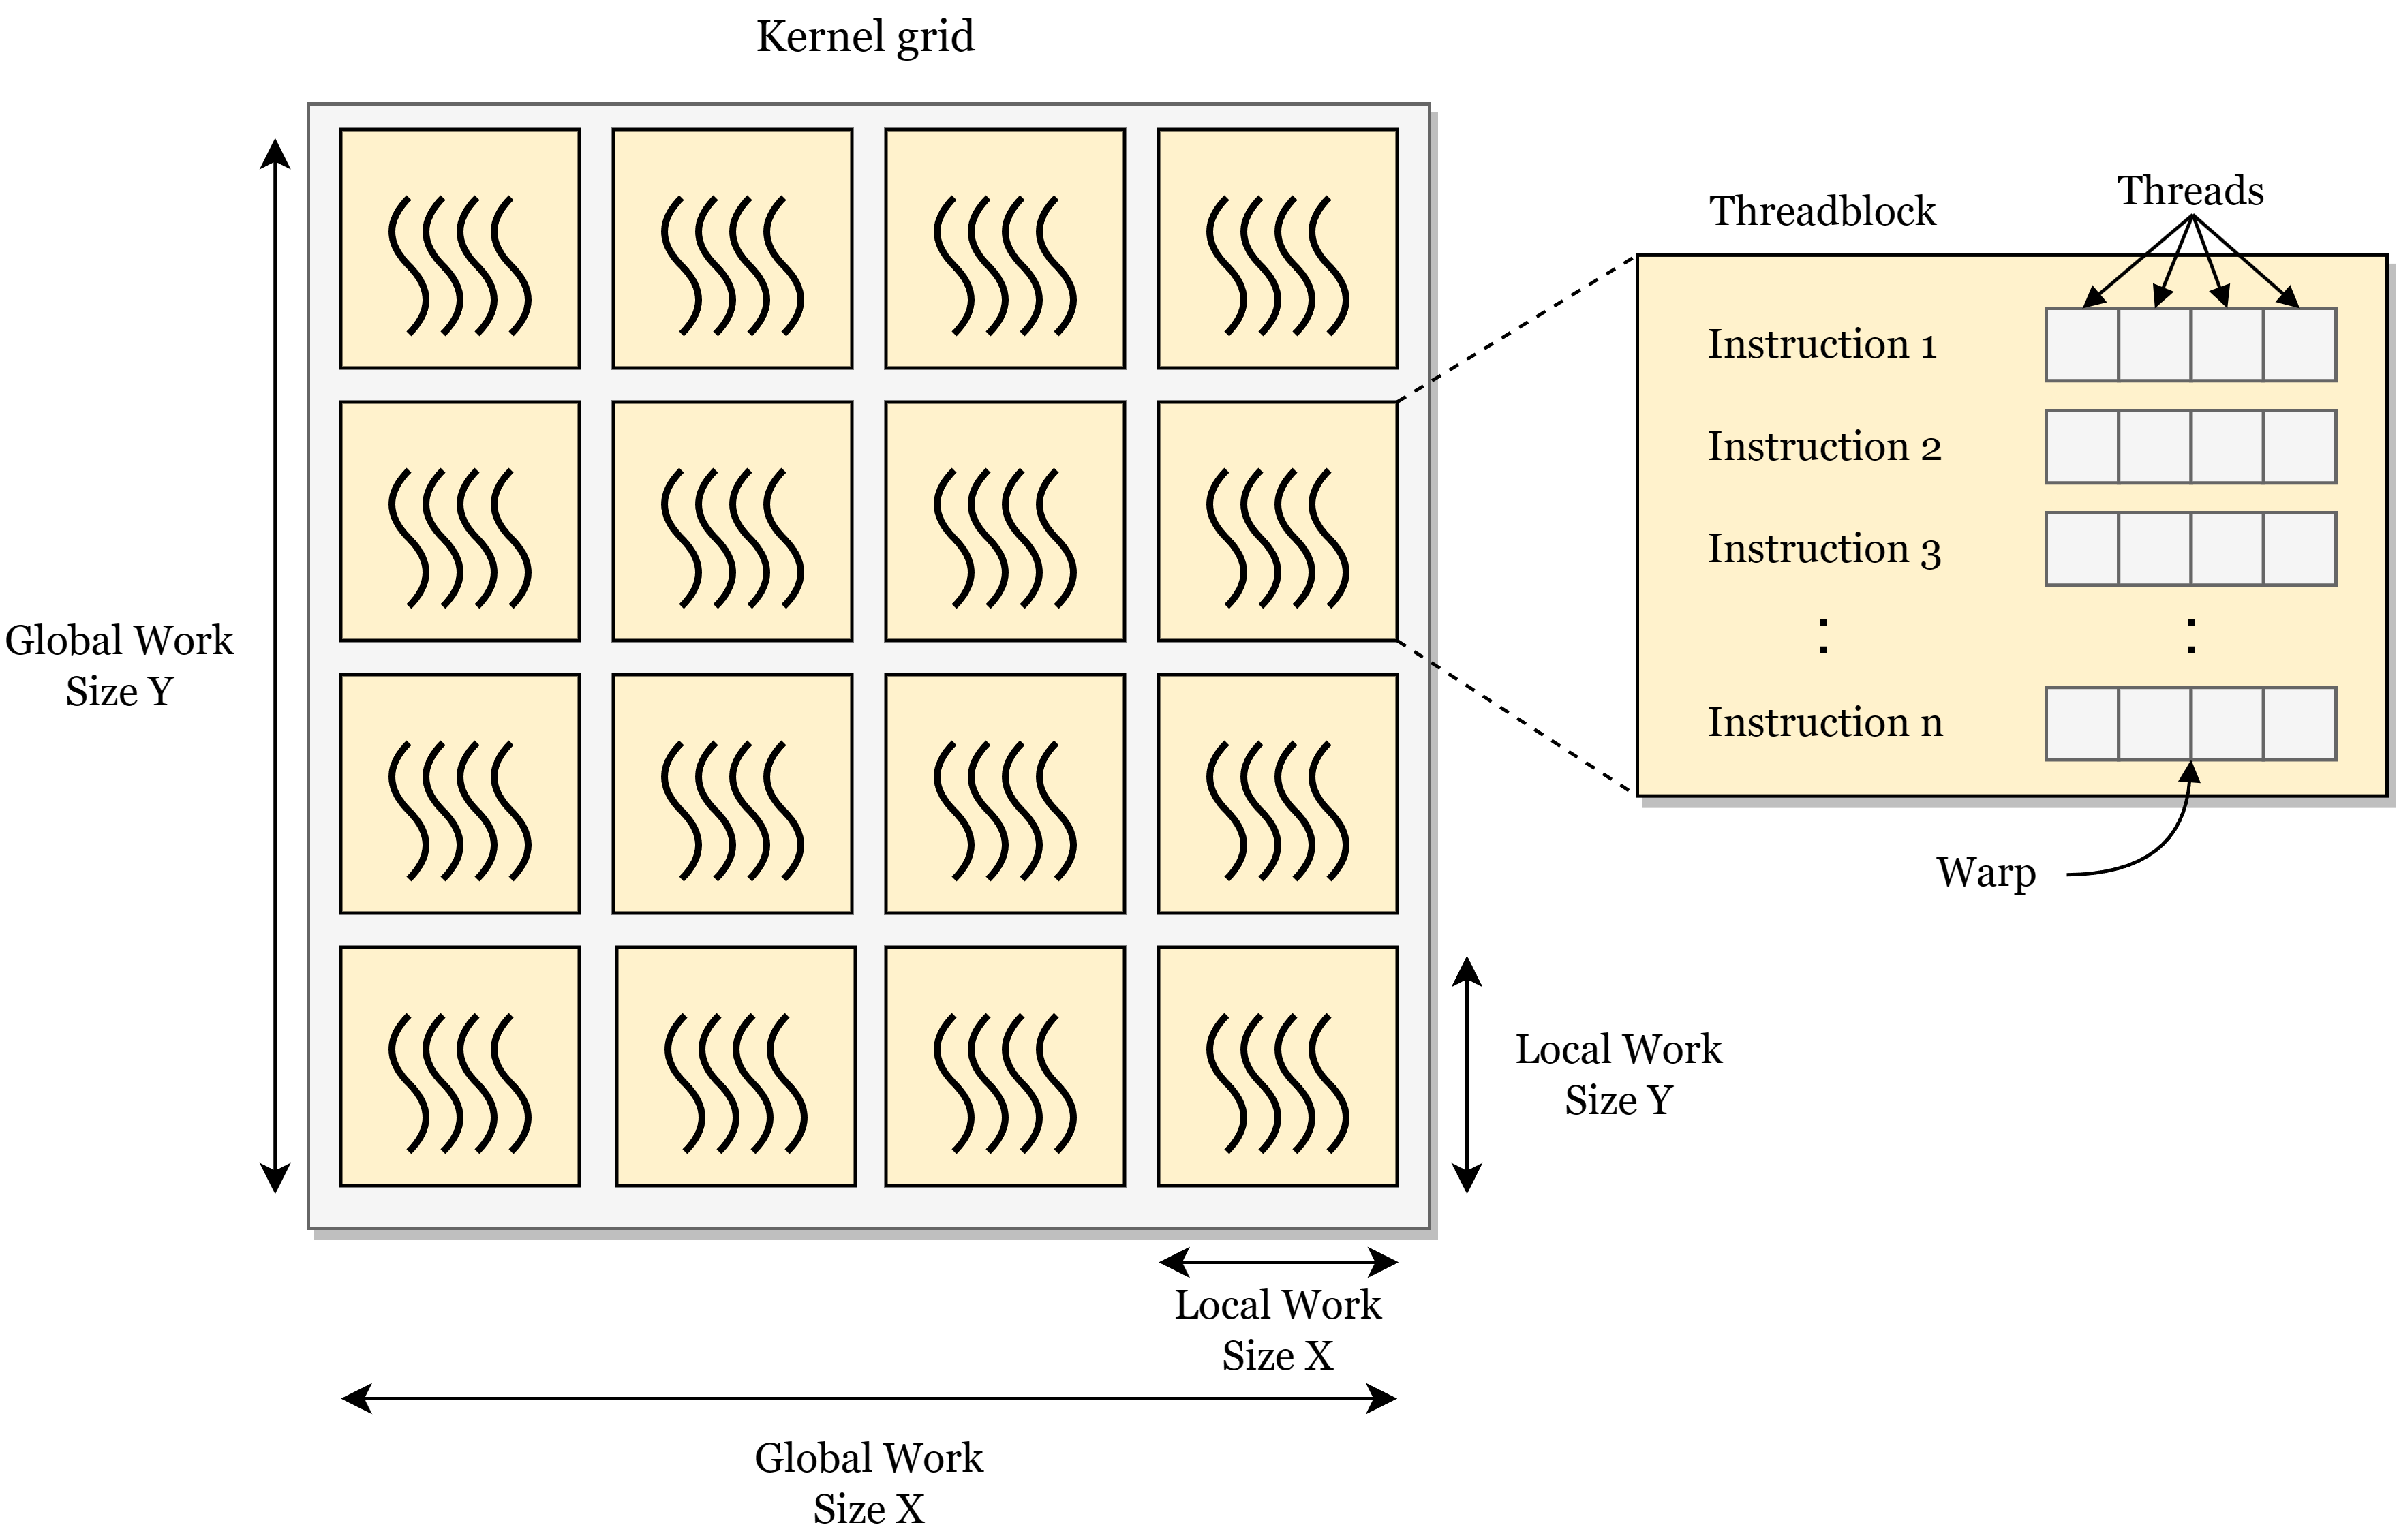
\includegraphics[width=0.9\textwidth]{figures/grid.png}
    \caption[Relating the kernel grid, warps and threads]{Illustration of how the kernel is divided into a grid of thread blocks, all containing a set number of threads running in lockstep. The threads all execute the same instructions, but on different data.}
    \label{fig:kernel_work_items}
\end{figure}

\begin{figure}
    \centering
    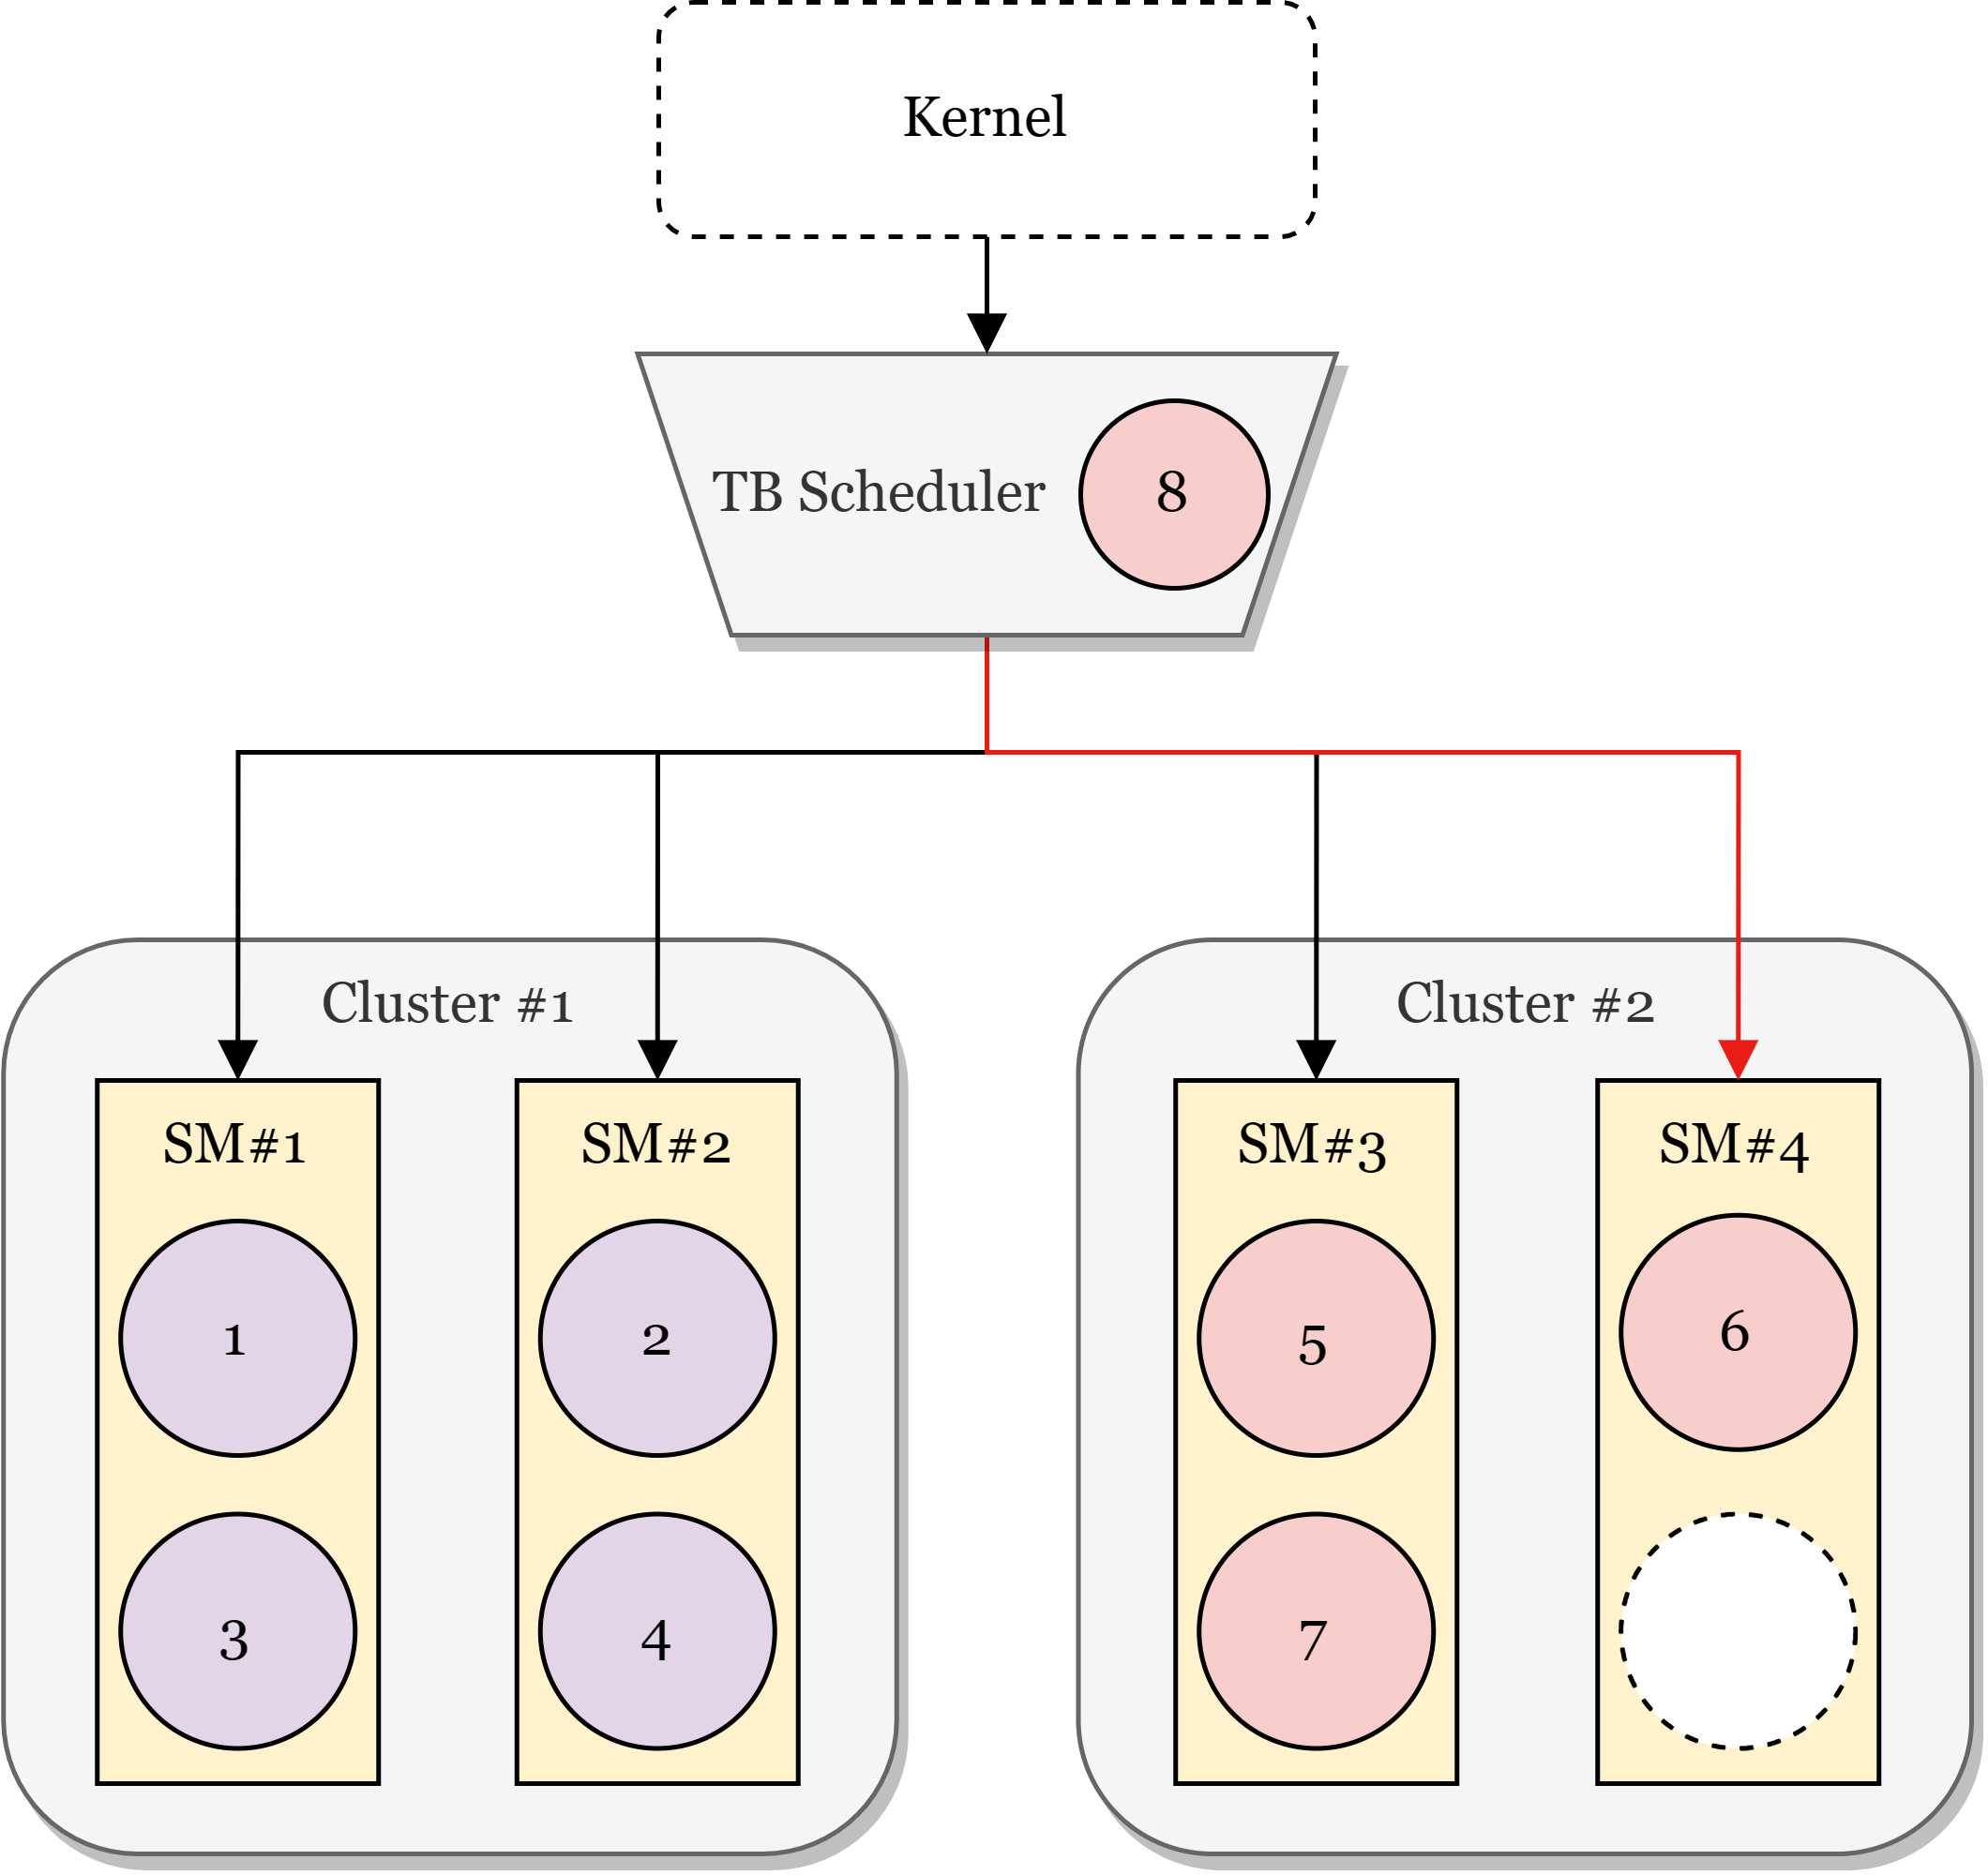
\includegraphics[width=0.6\textwidth]{figures/TB_scheduler.png}
    \caption[\acrshort{tb} scheduling]{Thread block scheduler scheduling \acrshortpl{tb} in a round-robin order among the \acrshortpl{sm} in the same cluster, but attempting to map neighbouring blocks to the same cluster to exploit locality.}
    \label{fig:tb_scheduler}
\end{figure}

% \begin{figure}
%     \centering
%     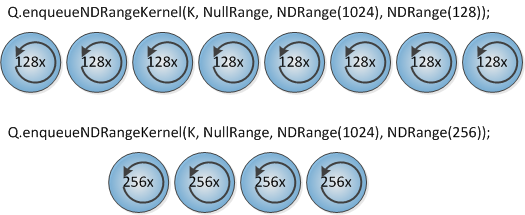
\includegraphics[width=0.8\textwidth]{figures/WG-vs-WI.png}
%     \caption{Work groups and work items (source)}
%     \label{fig:wg-vw-wi}
% \end{figure}

%\textcolor{red}{How the kernel is divided https://downloads.ti.com/mctools/esd/docs/opencl/execution/kernels-workgroups-workitems.html,
%https://registry.khronos.org/OpenCL/sdk/2.2/docs/man/html/clEnqueueNDRangeKernel.html}

\section{GPU Simulation} \label{sec:gpu_simulation}

\textcolor{red}{
In the spring of 2023, the Vortex team released Skybox \cite{skybox}, expanding upon \Gls{vortex}. They implemented a 3D graphics rendering accelerator supporting the Vulkan API, a modern graphics rendering API compared to the commonly used older OpenGL API. They also introduce a \Gls{riscv} \acrshort{isa} for accelerating graphics rendering, as well as implementing a compiler-driven control-flow divergence transformation to handle rendering loops inside graphics kernels. While \Gls{vortex} provides hardware texture units, Skybox has a hardware rasterizer and \acrfull{rop}. This results in a GPU more suitable for graphics workloads than \Gls{vortex}, as the \Gls{vortex} GPGPU is more suited towards compute workloads.}

GPGPU architecture research is mainly focused on using software simulations\cite{gem5_gpu}\cite{gpu_sim_cuda}\cite{multi2sim} modeling the architecture at the \acrfull{il} level such as PTX and HSAL. There are however significant deviations between GPU simulators using high-level abstractions and real hardware. Simulating IL instructions can add up to 33\% error when comparing the absolute runtimes to real hardware\cite{lost_in_abstraction}. High-level abstraction models have substantially less functional state associated with the instructions. Thus they are unable to model important micro-architectural interactions, such as instruction fetching and control divergence.

To obtain results reflecting the performance of an architecture most accurately, cycle accurate simulations are required. A solution to the inaccurate high-level abstraction simulations, is \acrfull{rtl} implementations. These implementations are cycle accurate, but require substantially more time and memory to simulate. This is because the entire state of the system is represented. There exists several \acrshort{rtl} implementations of open-source GPGPUs, such as MIAOW\cite{MIAOW}, Nyami\cite{Nyami} and FlexGrip\cite{FlexGrip}. 

Simulating entire systems in software is rather slow, especially for large multi-core systems as they are difficult to parallelize due to fine-grained synchronization\cite{graphite}\cite{wwt2}. To speed up architecture simulation, \acrshort{fpga}-acceleration can be used. RAMP-gold\cite{RAMP-gold}, an FPGA multicore simulator, achieved a $263\times$ speedup over GEMS\cite{gems}, a software based simulator. \acrshort{fpga}-acceleration serves as a middle ground between software simulation and \acrshortpl{asic}. As high-end \acrshortpl{fpga} are becoming more prevalent in the consumer market, implementing full-feature \acrshortpl{gpgpu} is becoming a possibility.

There is however a critical problem when running FPGA-accelerated simulations, modeling the timing and behaviour of I/O and peripherals\cite{chipyard}, e.g DRAM. To obtain representative results using \acrshort{fpga}-accelerated GPUs, both memory bandwidth and latency needs to be scaled to match the discrepancy between \acrshortpl{fpga} and \acrshortpl{asic}. Chipyard\cite{chipyard} is able to achieve this using Firesim\cite{firesim}. Firesim, use a token mechanism which can stall individual SoCs of the simulated system to advance the system in target time. 

\section{Warp Scheduling} \label{sec:warp_scheduling}

The warp scheduler and the scheduling algorithm can be integral to the performance of the GPU. Two commonly used warp scheduling algorithms are \acrfull{lrr} and \acrfull{gto} \cite{improving_gpgpu_scheduling}. Figure \ref{fig:lrr} and \ref{fig:gto} respectively illustrates how \acrshort{lrr} and \acrshort{gto} schedules warps. \acrshort{lrr} schedules warps in a round-robin order. If a warp is stalled, it is skipped, and the next warp can be scheduled. \acrshort{gto} selects the \acrshort{tb} with the oldest ready warp and schedules warps from the \acrshort{tb} until it stalls \cite{cache-conscious_wavefront_scheduling}. Other notable scheduling algorithms are CCWS\cite{cache-conscious_wavefront_scheduling}, CAWS\cite{caws} and LWS\cite{improving_gpgpu_scheduling}.

In the case of memory intensive applications, \acrshort{lrr} can cause situation where all warps arrive at long latency stalls at the same time as shown in Figure \ref{fig:lrr-lls} \cite{ZHANG2018520}. If all warps are stalled, the long latency stalls cannot be hidden, resulting in low throughput. Scheduling algorithms such as \acrshort{gto}, aims at reaching a stall for a single warp before scheduling others. This may enable more stalls to be hidden, as shown in Figure \ref{fig:gto-lls}, and even achieve better cache locality\cite{cache-conscious_wavefront_scheduling}\cite{ZHANG2018520}.

\begin{figure}
     \centering
     \begin{subfigure}[b]{0.45\textwidth}
         \centering
         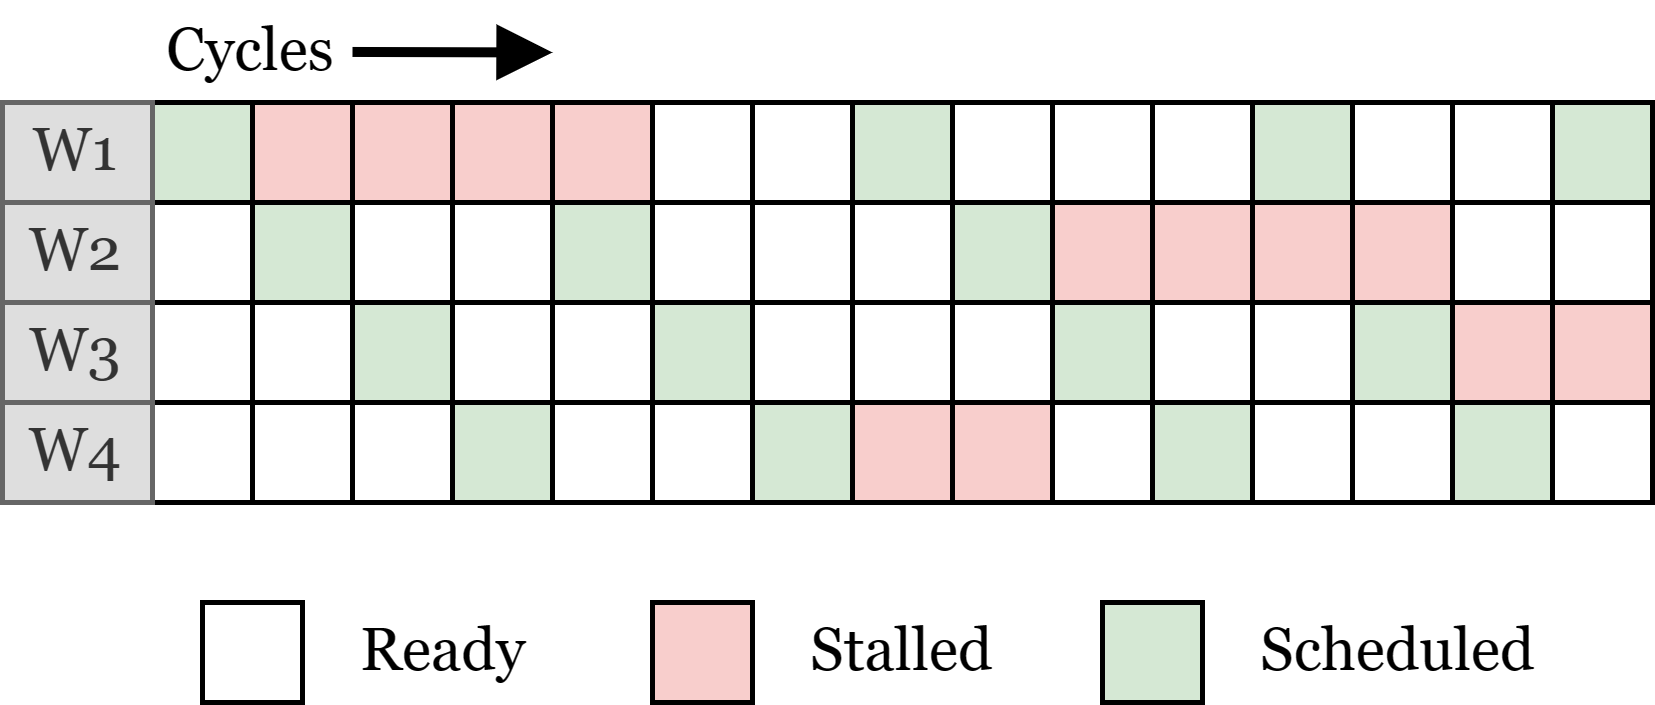
\includegraphics[width=\textwidth]{figures/warp-scheduling-lrr.png}
         \caption{Loose round-robin}
         \label{fig:lrr}
     \end{subfigure}
     \hfill
     \begin{subfigure}[b]{0.45\textwidth}
         \centering
         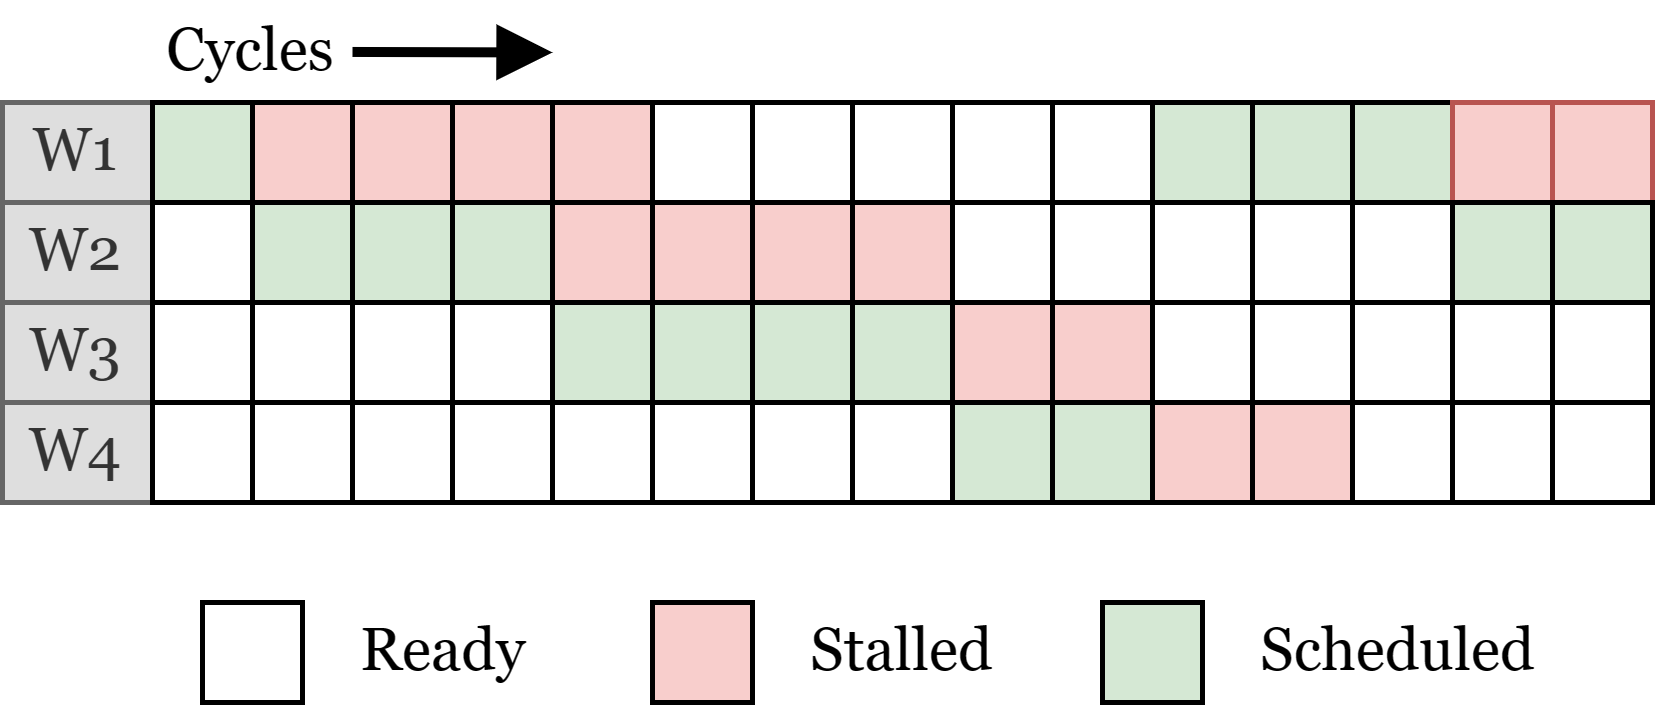
\includegraphics[width=\textwidth]{figures/warp-scheduling-gto.png}
         \caption{Greedy then oldest}
         \label{fig:gto}
     \end{subfigure}
    \caption{Demonstration of how LRR and GTO selects warps for scheduling}
    \label{fig:lrr_gto}
\end{figure}

\begin{figure}
     \centering
     \begin{subfigure}[b]{0.45\textwidth}
         \centering
         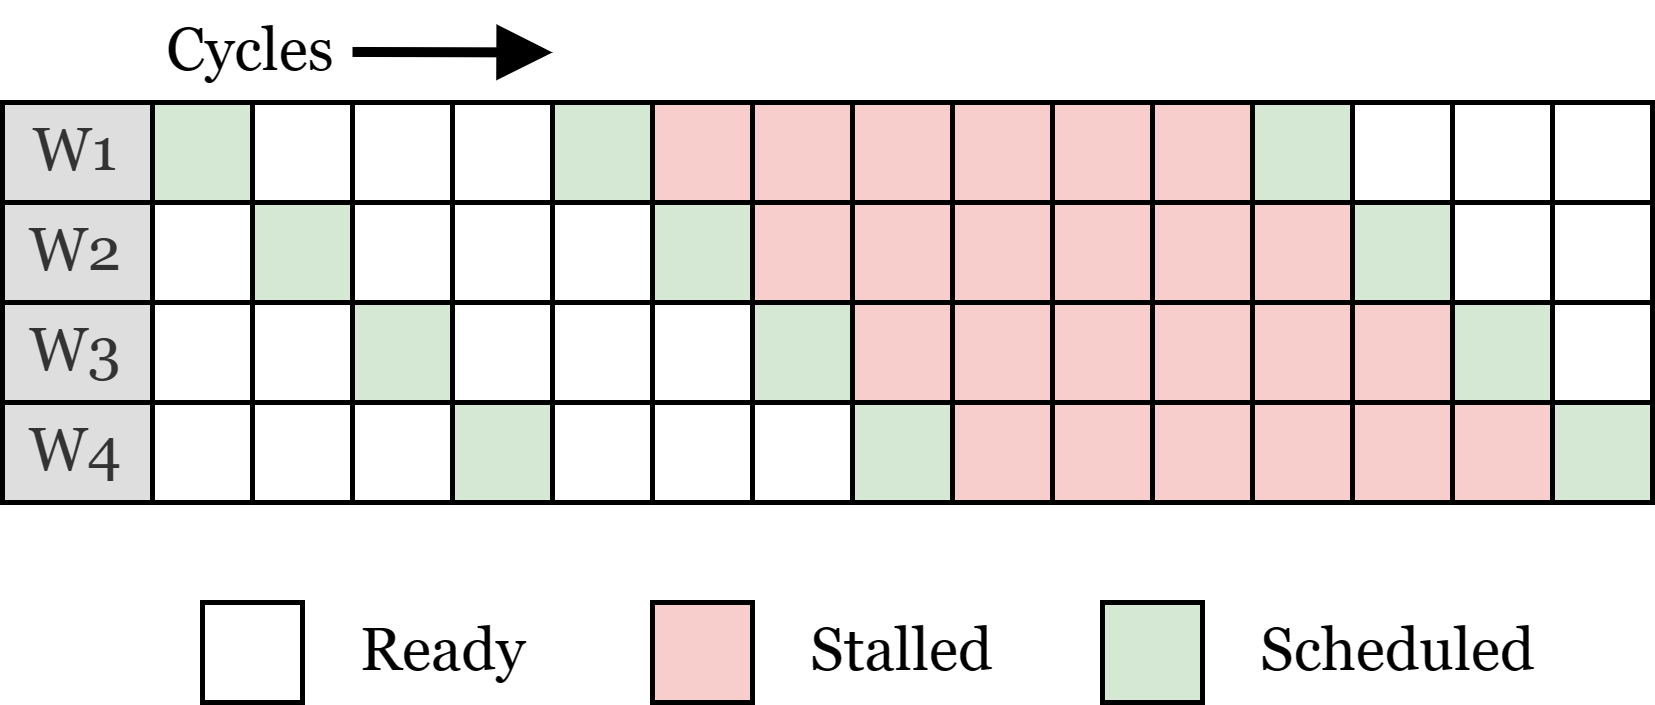
\includegraphics[width=\textwidth]{figures/warp-scheduling-lrr-stall.png}
         \caption{Loose round-robin}
         \label{fig:lrr-lls}
     \end{subfigure}
     \hfill
     \begin{subfigure}[b]{0.45\textwidth}
         \centering
         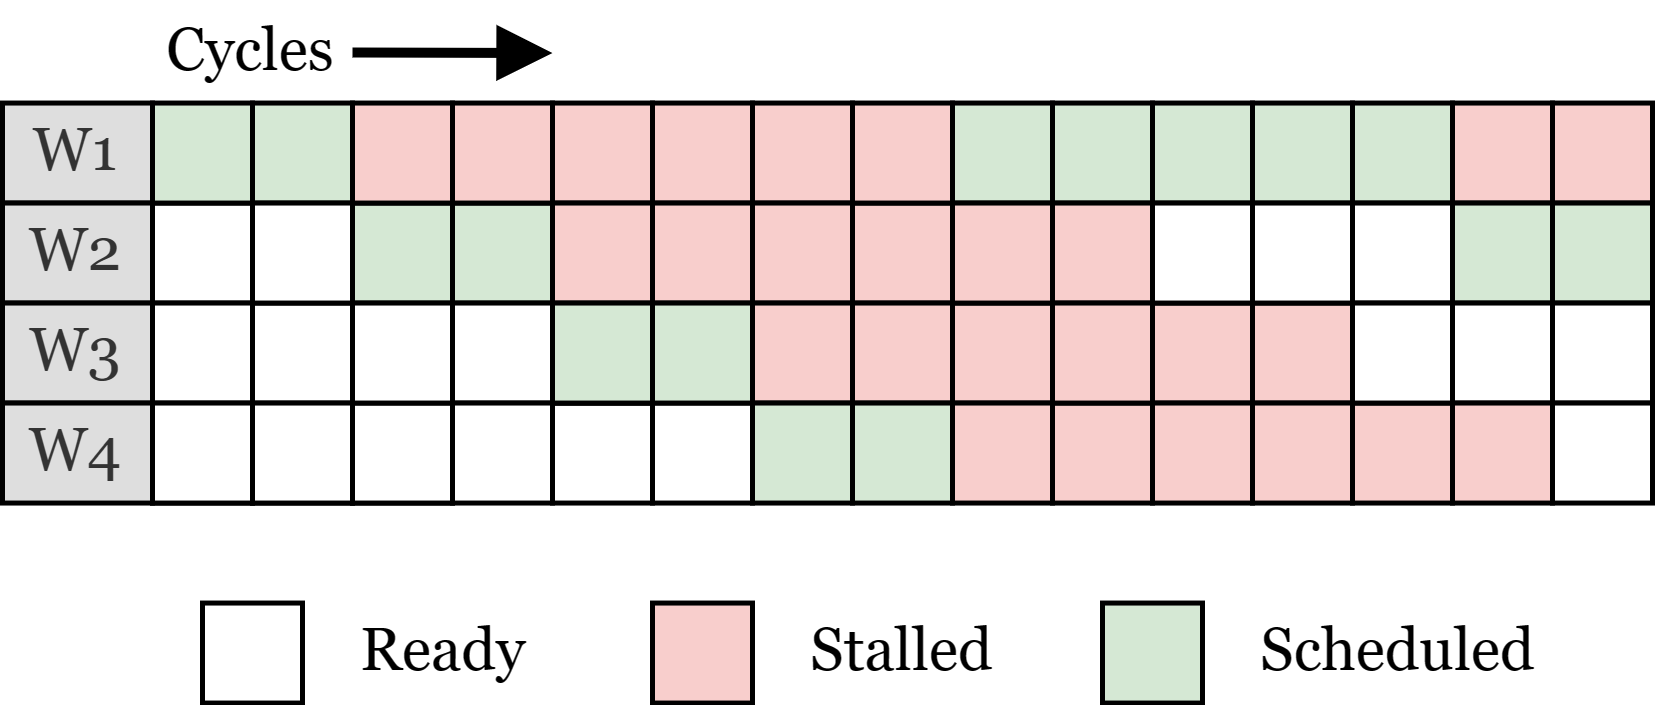
\includegraphics[width=\textwidth]{figures/warp-scheduling-gto-stall.png}
         \caption{Greedy then oldest}
         \label{fig:gto-lls}
     \end{subfigure}
        \caption[Demonstration of how \acrshort{lrr} and \acrshort{gto} handles long-latency stalls]{Demonstration of how \acrshort{lrr} and \acrshort{gto} performs in conjunction with long-latency stalls. \acrshort{gto} is able to hide the stalls, while \acrshort{lrr} is unable to because all warps stall at the same time}
        \label{fig:lrr-gto-lls}
\end{figure}

\section{Vortex}

Vortex\cite{vortex} is an open-source \gls{riscv} based \acrshort{gpgpu}. \Gls{vortex} supports OpenCL and can be simulated using \acrshort{fpga}-acceleration. Together with its customizable design and open-source compiler, driver and runtime, \Gls{vortex} aims to enable GPU architecture research. Vortex does however  not implement any mechanisms to scale memory latency or bandwidth as described in Section \ref{sec:gpu_simulation}. Work is currenly being done at NTNU's \acrfull{cal} to implement \Gls{vortex} into chipyard. Meanwhile, I have to use software simulation of \Gls{vortex} and DRAM to obtain representative results.

\subsection{Vortex' Software and Simulation Stack}

\Gls{vortex} has support for OpenCL and uses \Gls{pocl}\cite{pocl} to implement the compiler and runtime software for OpenCL. The \gls{pocl} runtime software provide an OpenCL interface between the host and \Gls{vortex}. The compiler have been modified to generate kernel binaries targeting the extended \gls{riscv} \acrshort{isa} used by \Gls{vortex}.

\Gls{vortex} allows for selecting between a set of different simulation environments, which are displayed in Figure \ref{fig:simstack}. The available environments are the OPAE driver, VLSIM, RTLSIM and SIMX. The OPAE driver makes use of Intel's propretary AFU simulation environment (ASE). Both VLSIM and RTLSIM utilize Verilator to simulate the RTL design and use Ramulator\cite{Ramulator}, an extensible DRAM simulator providing cycle-accurate performance models, to simulate memory in software. VLSIM additionally simulates the AFU in software. The SIMX driver implements a cycle-level simulator for \Gls{vortex}. All of these drivers share a common API when executing programs. 

To simulate \Gls{vortex} using RTLSIM (or VLSIM), Verilator\cite{verilator} is used to compile the SystemVerilog implementation of \Gls{vortex} into a vortex library, which can simulate the the entire \acrshort{gpu} cycle-accurately. When executing a program, it is linked with the \Gls{vortex} driver and \Gls{vortex} library generated by Verilator. This allows the host to treat the simulated \acrshort{gpu} as if it was a normal \acrshort{gpu} using an OpenCL interface.

% Presentation by vortex group 
% https://www.youtube.com/watch?v=h1xDQILSZnI&ab_channel=MICROSymposium

\begin{figure}
    \centering
    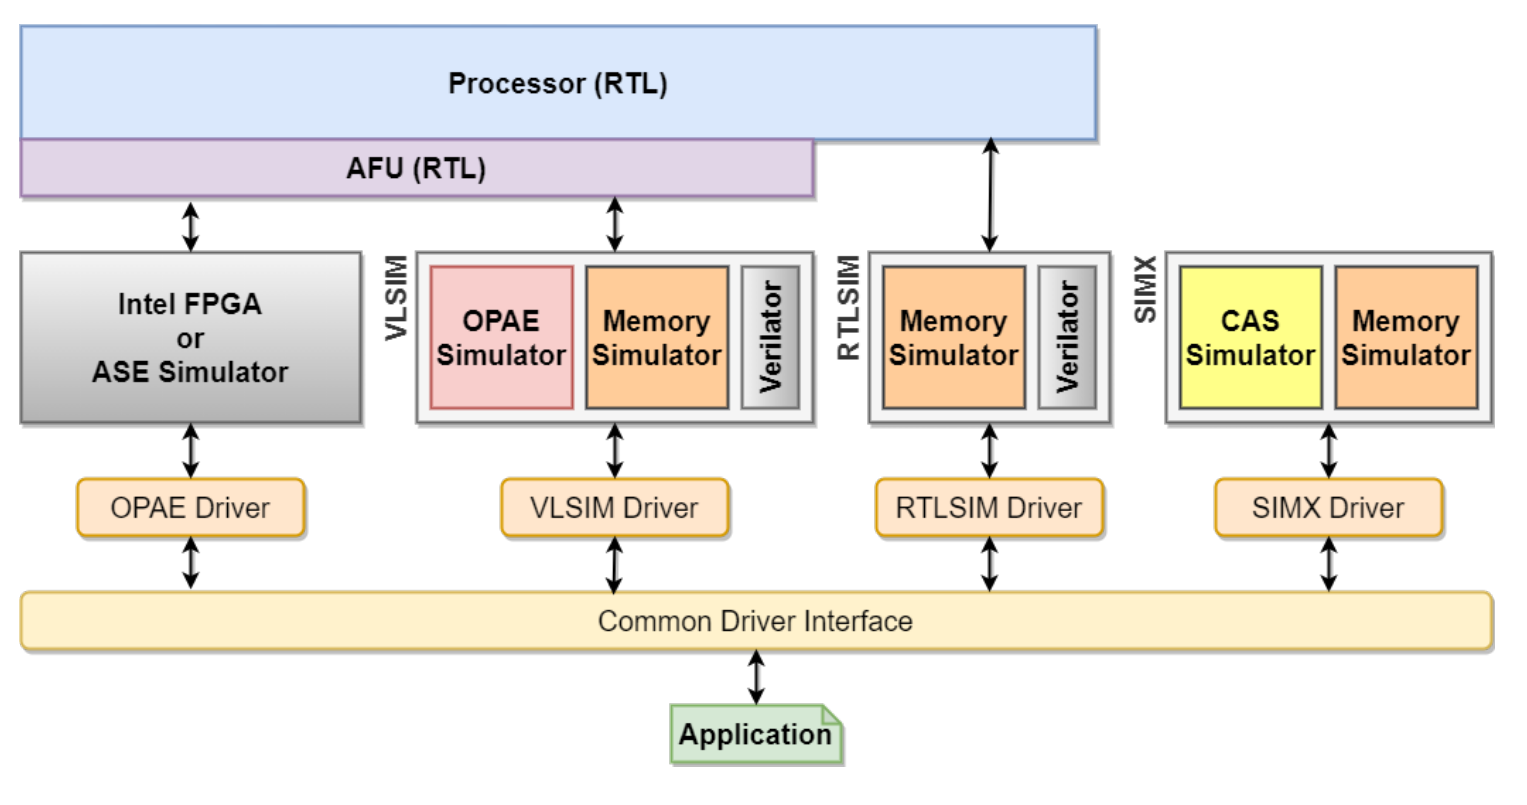
\includegraphics[width=0.8\textwidth]{figures/simstack.png}
    \caption[Vortex simulation stack]{Vortex simulation stack reproduced from \cite{vortex}.}
    \label{fig:simstack}
\end{figure}

\subsection{Instruction set}

Vortex extends the \gls{riscv} \acrshort{isa} \cite{riscv-isa} with six new instructions, which are listed below.
\begin{itemize}
    \item \textbf{wspawn}: Controlling warps by activating a number of warps at a specified \acrshort{pc}.
    \item \textbf{tmc}: Controlling threads by activating or deactivating threads within a warp. 
    \item \textbf{split \& join}: Handling control divergence. \textit{Split} pushes information about the current state of the thread-mask and branching to the \acrfull{ipdom} stack, and \textit{join} pops the information off the stack to reconverge the branches.
    \item \textbf{bar}: Synchronizing warps, both intra-core and inter-core, using barriers. The barrier is released when the expected number of warps has reached it.  
    \item \textbf{tex}: Texture lookup with a variety of configurable features, such as mipmapping. 
\end{itemize}
